\documentclass{beamer}

\usepackage{beamerthemesplit}

\usepackage[utf8]{inputenc}
\usepackage[russian]{babel}
\usepackage{amsmath,amsfonts,amsthm,amssymb,thmtools}
\graphicspath{ {Images/} }

% Good footer
\addtobeamertemplate{navigation symbols}{}{%
    \usebeamerfont{footline}%
    \usebeamercolor[fg]{footline}%
    \hspace{1em}%
    \insertframenumber/\inserttotalframenumber
}

\newcommand{\eqnref}[1]{\eqref{#1}}
\newcommand{\secref}[1]{Section \ref{#1}}
\newcommand{\figref}[1]{Figure \ref{#1}}
\newcommand{\lemref}[1]{Lemma \ref{#1}}
\newcommand{\corref}[1]{Corollary \ref{#1}}
\newcommand{\thmref}[1]{Theorem \ref{#1}}
% Real numbers
\newcommand{\Real}[1]{\mathbb{R}^{#1}}
% Complex numbers
\newcommand{\Complex}[1]{\mathbb{C}^{#1}}
% Integers
\newcommand{\Integer}[1]{\mathbb{Z}^{#1}}
% Rank operator
\DeclareMathOperator{\rank}{\textnormal{rank}}
% Vec operator
\newcommand{\vecop}{\textnormal{vec}}
% Norm
\newcommand{\norm}[1]{\left|\left|#1\right|\right|}
% Trace
\newcommand{\trace}{\textnormal{tr}}
% Range
\newcommand{\range}{\textnormal{range}}
% Partial derivative
\newcommand{\pd}[2]{\dfrac{\partial #1}{\partial #2}}
% Complete derivative
\newcommand{\dd}[2]{\dfrac{d #1}{d #2}}
% Complete derivative, second order
\newcommand{\dds}[2]{\dfrac{d^2 #1}{d {#2}^2}}
% Limit to N / N
\newcommand{\limover}[1]{\lim_{#1 \rightarrow \infty} \dfrac{1}{#1}}
% Display style sum
\newcommand{\dsum}{\displaystyle\sum}
% arg min and arg max
\newcommand{\argmax}[1]{\underset{#1}{\operatorname{arg~max}}}
\newcommand{\argmin}[1]{\underset{#1}{\operatorname{arg~min}}}
%---------------------------------------------------------------------------
% Create theorem without number
\declaretheoremstyle[headfont=\bfseries,notefont=\bfseries,bodyfont=\itshape,notebraces={}{},headpunct={},postheadspace=1em]{mystyle}
\declaretheorem[style=mystyle,numbered=no,name=Теорема]{thm-hand}

\theoremstyle{plain}
\newtheorem{thm}{Теорема}
\newtheorem{lem}[thm]{Лемма}
\newtheorem{state}[thm]{Утверждение}
\newtheorem{cor}[thm]{Следствие}
\newtheorem{conj}[thm]{Предположение}
\newtheorem{rmk}[thm]{Замечание}
\newtheorem{proof-rus}[thm]{Доказательство}
\newtheorem{obs}[thm]{Наблюдение}
\newtheorem{dfn}[thm]{Определение}
\theoremstyle{definition}
\newtheorem{Q}[thm]{Вопрос}
\newtheorem{A}[thm]{Ответ}
\newtheorem{prob-rus}[thm]{Задача}
\newtheorem{ex}[thm]{Пример}

\usetheme{Warsaw}

\title{Лекция 9}
\author{Подготовил Чижов Даниил, КН-302}

\begin{document}
\date{16.11.15}

\frame{\titlepage
\begin{center}
Теория алгоритмов 2015
\end{center}
}


\section{Лектор - Юрий Окуловский}

\begin{frame}
    \begin{center}
        \textbf{N = NP?} \\
        (Можно ли решить огромное количество важных задач за разумное время?)
    \end{center}
\end{frame}

\begin{frame}
    \begin{itemize}
        \item { Да }
        \item { Нет }
        \item { Не знаю и не могу знать }
        \item { Все равно }
    \end{itemize}
\end{frame}

\begin{frame}
    Дальше будем предполагать, что $P\neq NP$ \\
    Рассмотрим классы функциональных задач $FP$ и $FNP$
    \begin{prob-rus}
        Задача поиска $R=\left \{ (x,y)|x,y \in \sum \right \}$.
    \end{prob-rus}
    \begin{dfn}
        $R \in FP \Rightarrow \exists$ ДМТ, которая по $x$ вычисляет $y: \; (x,y) \in R$ за полином. \\
        $R \in FNP \Rightarrow \exists$ НМТ, которая по $x$ вычисляет $y: \; (x,y) \in R$ за полином.
    \end{dfn}
\end{frame}
    
\begin{frame}
    \begin{dfn}
        $R \in FNP \Rightarrow \exists$ ДМТ $M_{R}$, которая за полином проверяет, что $(x,y) \in R$.
    \end{dfn}
    То есть, умеет быстро проверять, что $y$ является ответом для $x$.
    \begin{prob-rus}
        $F-SAT$ : по $F$ найти $x_{1}, .., x_{n}: \; F(x_{1}, .., x_{n})=1$.
    \end{prob-rus}
\end{frame}

\begin{frame}
    \begin{dfn}
        Сводимость по Куку $\underset{p}{\rightarrow}$. \\
        $R_{1} \; \underset{p}{\rightarrow} \; R_{2}$, если $\exists$ МТ для задачи $R_{1}$, которая использует оракул $R_{2}$ и работает за полином.
    \end{dfn}
    \begin{dfn}
        Оракул $R_{2}$ - это гипотетическое устройство, решающее $R_{2}$ за 1.
    \end{dfn}
    \begin{rmk}
        Сводимость по Карпу - это частный случай сводимости по Куку.
    \end{rmk}
    То есть, если что-то свелось по Карпу, то оно свелось и по Куку. Обратное не верно.
\end{frame}

\begin{frame}
    $F = \begin{matrix} x_{1} \vee \bar{x_{2}} \vee x_{3} \\ 
    x_{1} \vee x_{2} \vee \bar{x_{3}} \\ ......... \end{matrix}$ \\
    \begin{prob-rus}
        $F-SAT$: по $F$ найти $x_{i}, \; F(x_{i})=1$
    \end{prob-rus}
    Оракул решает задачу $SAT$ за 1. Мы ей говорим формулу $F$, а она отвечает Да или Нет.
    \begin{dfn}
        $F|_{x_{1}}$- выполнима $\Leftrightarrow \; \exists x_{1}, .., x_{n}: F(x_{1}, .., x_{n})=1 \wedge x_{1}=1$
    \end{dfn}
\end{frame}

\begin{frame}
    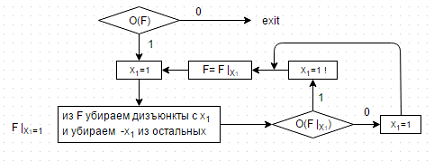
\includegraphics{scheme1}
\end{frame}

\begin{frame}
    \begin{dfn}
        Сводимость по Левину $\underset{l}{\rightarrow}$. \\
        $R_{1} \; \underset{l}{\rightarrow} \; R_{2}$, если $\exists \; f,g$- полиномиально вычислимые полиномиальные функции и $(x, g(y)) \in R_{1} \Leftrightarrow (f(x), y) \in R_{2}$. \\
        $f$ - преобразует задачу $R_{1}$ к $R_{2}$,\\
        $g$ - преобразует ответ.
    \end{dfn}
    Если бы мы сводили по Левину задачу $F-3SAT$ к задаче $F\_VC$, то выполнили бы следующие действия: \\
    $F \rightarrow Graph \rightarrow VC \rightarrow x_{1}, .., x_{n}: \; F(x_{1}, .., x_{n})=1$. \\ То есть все сведения, которые мы делали, - это сведения по Левину. \\
    \begin{rmk}
        Сводимость по Левину - это обобщение сводимости по Карпу для функциональных задач.
    \end{rmk}
\end{frame}

\begin{frame}
    $F = \begin{matrix}x_{1} \vee x_{2} \vee \bar{x_{3}} \\ 
    \bar{x_{1}} \vee x_{2} \vee x_{3} \\ x_{1} \vee x_{2} \vee x_{3} 
    \end{matrix} \overset{f}{\rightarrow}$ \\
    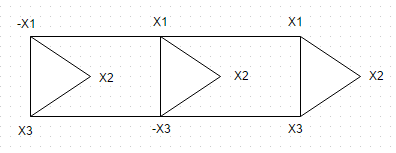
\includegraphics{scheme2} \\ $\rightarrow \begin{Bmatrix} x_{2}\\ x_{2}\\ x_{2} \end{Bmatrix} \overset{g}{\rightarrow} \begin{matrix} x_{2}=1\\ x_{1}=0\\ x_{3}=0 \end{matrix}$
    
\end{frame}

\begin{frame}
    \begin{dfn}
        $R \in FNP$ - трудная $\Leftrightarrow \forall R'\in FNP \underset{l}{\rightarrow} R$.
    \end{dfn}
    \begin{dfn}
        $R \in FNP$ - полная $\Leftrightarrow R\in FNP$ - трудная и $ R\in FNP$.
    \end{dfn}
    \begin{dfn}
        Самосводимые задачи.
        $FNP$-полные задачи всегда сводятся по Карпу к своим $NP$-полным аналогам.
    \end{dfn}
    \begin{dfn}
        Decision version.
        $R={(x,y)}$ \\
        $L_{R}= \left \{ x: \; \exists y: (x,y) \in R \right \}$
    \end{dfn}
\end{frame}

\begin{frame}
    \begin{state}
        Все $FNP$-полные задачи самосводимы.
    \end{state}
    \begin{proof-rus}
        $R \; \underset{l}{\rightarrow} \; F-SAT \; \underset{p}{\rightarrow} \; SAT \; \underset{k}{\rightarrow} \; Decision \; version \; R$ \\
        Алгоритм: \\
        1. Берем $R$ и переводим его в формулу $F$ из задачи $F-SAT$. \\
        2. Мы знаем, что $F-SAT \; \underset{p}{\rightarrow} \; SAT$. Запускаем этот алгоритм. \\
        3. Каждый вызов $O(F)$ заменяем на вызов $O_{L_{R}}(h(F))$. \\
        4. $return \; g($решение $F-SAT)$.
    \end{proof-rus}
\end{frame}

\end{document}